\documentclass[../main.tex]{subfiles}
\begin{document}
\chapter{The stationary solution space}\label{chapter5}
In this final chapter, we take the solutions for wind and expanded envelopes from the previous two chapters and combine them to analyze the total solution space of PRE bursts. We are interested in the qualitative differences between the profiles of the solutions (\S\ref{sec:compare_profiles}), and quantitative differences in the observables, mainly the luminosities and photospheric radii. In \S\ref{sec:compare_Lb}, we establish timescales for the solutions to determine if steady-state solutions are truly appropriate for describing the evolution of PRE bursts. We conclude in \S\ref{sec:compare_photosphere_def} by analyzing how the different definitions for the photosphere for winds and envelopes might affect our results.

\section{Profiles}\label{sec:compare_profiles}
While we have already shown radial profiles of winds in Chapter 3 and envelopes Chapter 4, it is instructive to plot some of them together to analyze the general differences between the two regimes. 

\begin{figure}[htb!]
    \centering
    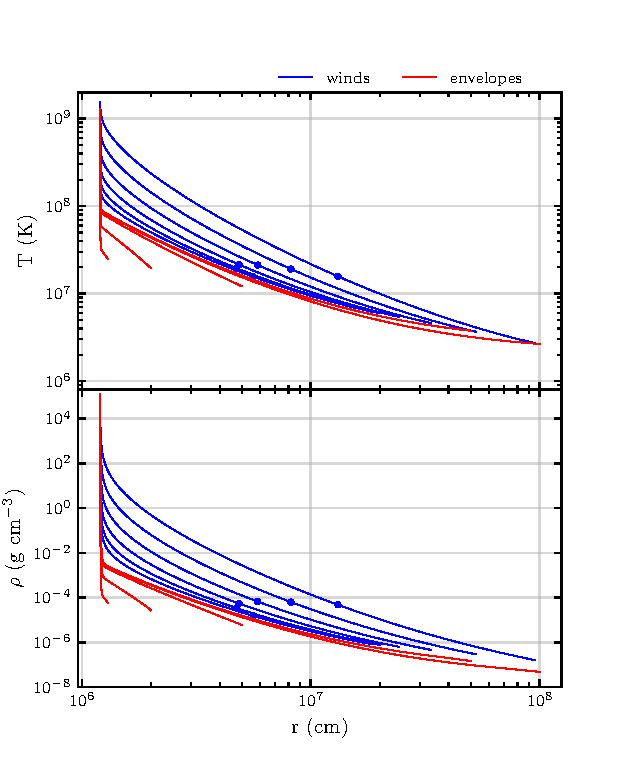
\includegraphics{figures/profiles.pdf}
    \caption[Radial profiles of winds and envelopes]{Temperature and density radial profiles for wind and envelope models.  Dots indicate the position of the wind critical points.  The mass-loss rates for the winds are $\log\dot{M}=19.0,18.5,18.0,17.5$  g s$^{-1}$, and the photospheric radii for the envelopes are $r\ph=13,20,50,100,500,1000$ km.}
    \label{fig:radial_profiles}
\end{figure}

In Fig.~\ref{fig:radial_profiles}, we show the temperature and density profiles for a few wind and envelope models.  Close to the surface, the sharp drop in temperature is associated to a drop density in both regimes. This region corresponds to a thin layer in hydrostatic equilibrium, even in the winds where the velocities are initially very low. This suggests a natural transition mechanism between the two regimes. At the onset of the burst, while the luminosity is rising towards the $\Ledd$, the envelope could expand hydrostatically, and only start to outflow from the upper layers as $L_b
^\infty$ eventually crosses $\Ledd$, pushing the photosphere from tens to hundreds of km. The opposite could happen at the end of the PRE phase of the burst, where the wind could eject its upper layers before dying out, leaving behind the still-expanded static envelope. 

We can also see in Fig.~\ref{fig:radial_profiles} that there are degeneracies between the static envelope and outflowing wind cases in terms of the radius of the photosphere and its temperature. For instance, the $\Mdot=10^{18.5}$ g s$^{-1}$ wind and $r\ph=1000$ km envelope have photospheres at similar radii and temperatures (but different densities). This suggests that there could be confusion from an observer's standpoint on which expansion regime is truly being observed. However, we will show later in this chapter that the timescales of these very extended envelopes and the narrow range of base luminosities that produce them make them unlikely to form during bursts. 

Fig.~\ref{fig:rho_T} shows the solution space in the density-temperature space. We have already analyzed these thoroughly in previous chapters, but it is interesting to note that the transition to a gas pressure dominated regime happens at much smaller densities for the envelopes than for the winds. This can be explained by the smaller luminosity, requiring a bigger contribution from the gas in order to hold up the envelope.

\begin{figure}[htb!]
    \centering
    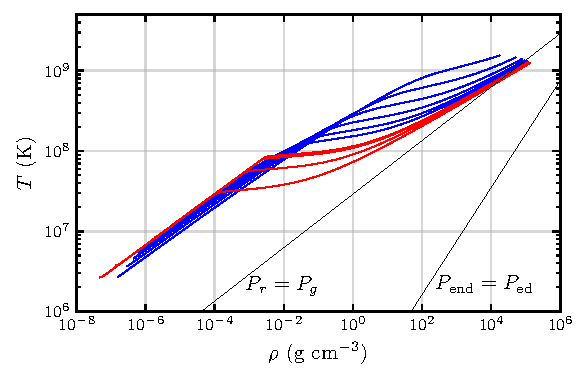
\includegraphics{figures/rho_T.pdf}
    \caption[Temperature-density profiles of winds and envelopes]{Temperature-density profiles for wind and envelope models. The models are the same as in Fig.~\ref{fig:radial_profiles}}
    \label{fig:rho_T}
\end{figure}

\section{Base luminosity}\label{sec:compare_Lb}
This section revolves around Fig.~\ref{fig:triple}, which is the main result of this work. By looking at various quantities from both regimes as a function of the base luminosity, we can assess the transition between the both regimes more clearly, as it is this parameter which connects the evolution of the burning layer throughout the burst to the extended structures. 

In the first panel, we plot the base temperature. As a reminder, this \textit{base} is defined in the same way for both winds and envelopes, where a fixed column depth (or equivalently pressure) is set at the stellar radius. In this way, we are truly comparing the state of the base at the same point. We see that the envelopes only represent a tiny portion of the flux-temperature profile at the base. There is also a gap in flux between the two regimes. For reasons that were explained in Chapter 3, we were not able to compute wind models with mass-loss rates lower than $10
^{17.15}$ g s$^{-1}$. But looking at the behavior of the curves, it is natural to think that  if we were able to improve our numerical method, then the envelope and wind models would join up smoothly at the base. In fact, this is completely expected, since the base is in hydrostatic equilibrium in both regimes, so that the flux-temperature profile is essentially just a direct consequence of the chosen EOS. Lastly, we see that winds with high mass-loss rates approach the radiation temperature limit, which is the temperature for which all of the pressure, a constant $P=gy$ because of the boundary condition \ref{eq:wind_innerBC}, is equal to the radiation pressure $U_R/3$, meaning that the gas is in a completely radiation pressure dominated regime. This temperature can be written as
\begin{align}\label{eq:Trad}
    T_\text{rad}=1.5\times 10^9\text{ K}&\left(\frac{M}{1.4\Msun}\right)^{1/4}\left(\frac{R}{12\text{ km}}\right)^{-1/2}\left(\frac{y}{10^8 \text{ g cm}^{-2}}\right)^{1/4}\nonumber\\
    &\left[1-0.35\left(\frac{M}{1.4\Msun}\right)\left(\frac{12\text{ km}}{R}\right)\right]^{-1/8}\,,
\end{align}

\newpage

\begin{figure}[H]
    \centering
    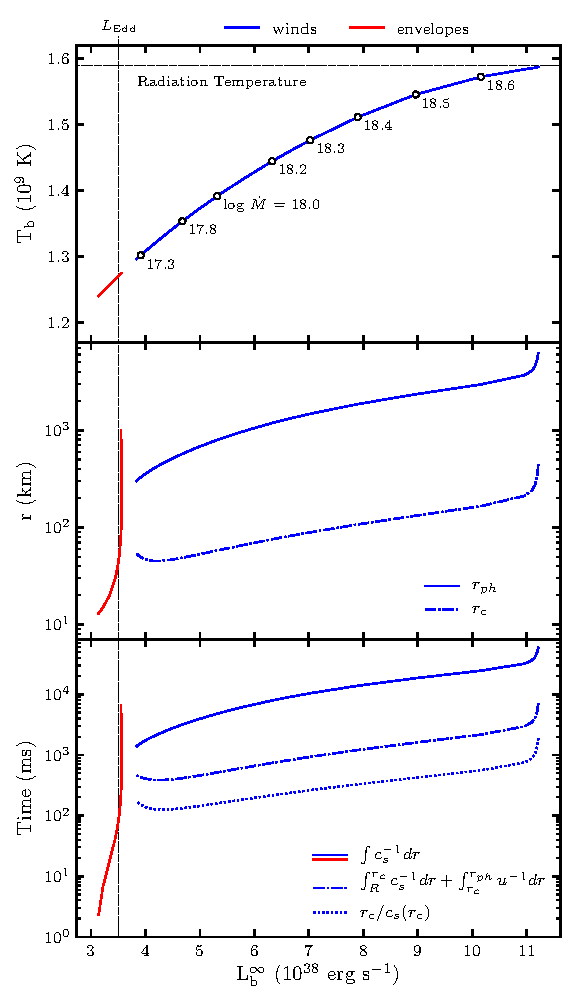
\includegraphics{figures/triple.pdf}
    \caption[Solution space for the base luminosity]{Solution space for the base luminosity as seen by observers at infinity, for both winds (blue) and envelopes (red).  Eddington luminosity is marked by the vertical black dashed line. \textit{Top}: Temperature at the base.  Mass-loss rates are indicated at various points for the winds.  \textit{Middle}: Photospheric and critical point radii.  \textit{Bottom}: Characteristic timescales of the solutions from the base to the photosphere (see text).}
    \label{fig:triple}
\end{figure}

\newpage

\noindent where $y$ is the chosen fixed column depth at the base of the wind. This shows that the radiation temperature is not very high in this context, and that any calculation of wind models is bound to approach this limit at high $\Mdot$, even with different neutron star parameters or inner boundary condition. 

While the static to outflowing transition seems to be smooth when looking at the base, it clearly is not if we study the extended regions, and in particular the photosphere, as can be seen in the second panel of Fig.~\ref{fig:triple}. Indeed, there is a clear discontinuity just above $\Ledd$, since envelope models with near-Eddington luminosities shoot up in terms of photospheric radius, instead of leveling off to the values of low $\Mdot$ wind models. This indicates that it is not possible to transition from one regime to the other in a quasi-static way, i.e by going from one stationary solution to the other when changing the base flux.  While both regimes may exist for some time if the base flux remains close to constant, the transition can only be modelled by fully time-dependent hydrodynamical calculations.  

Furthermore, while our models are all analytic solutions to stationary equations, we must ensure that the luminosity evolves slowly enough that the system is in fact able to reach a steady-state, and progress from one solution to the next.  We look at characteristic timescales in the third panel of Fig.~\ref{fig:triple} to determine if this could be the case.  The natural timescale for static structures is the sound crossing time
\begin{equation}
    \tau_\text{sound}=\int_R^{r\ph}c_s^{-1}dr\,,
\end{equation}
which gives the time taken for a sound wave to travel the structure, from the base to the photosphere. For winds, other natural timescales are the sound crossing time for one critical point
\begin{equation}
    \tau_\text{cr}=\frac{r_c}{c_s(r_c)}\,,
\end{equation}
and the flow crossing time
\begin{equation}
    \tau_\text{flow}=\int_R^{r\ph}u^{-1}dr\, .
\end{equation}
The problem with the latter is that the velocity is so small near the surface that the flow time is dominated by these regions, and therefore not representative of the whole solution. Instead, we take a timescale that combines the sound crossing time of hydrostatic regions, up to the critical point, followed by the flow crossing time in the outflowing regions of the wind, up to the photosphere:
\begin{equation}
    \tau_\text{sound-flow}=\int_R^{r_c}c_s^{-1}dr + \int_{r_c}^{r\ph}u^{-1}dr \,.
\end{equation}
Fig.~\ref{fig:triple} shows that these wind timescales have similar values and progressions with $L_b$, except for low mass-loss rates where the increase in critical point radii results in larger crossing times. 

In every model, by looking at the bottom two panels in Fig.~\ref{fig:triple}, it is clear that it is the photospheric radius which largely dictates the timescales. This means that more extended structures take longer to form, and that they cannot exist under a rapidly varying luminosity. Typical bursts have a rising phase of $\sim1$ s, a super-Eddington or PRE phase of $\sim10$ s and a decaying phase of $\sim1$ min.  Since the rising phase is so fast in transitioning from sub to super-Eddington luminosities, it is clear that our stationary solutions are not appropriate for describing its dynamics. However, the timescales would allow for PRE and decaying phase to be reasonably be modelled by stationary winds and envelopes respectively, except for the transition from super to sub-Eddington luminosities in the decay.  Finally, the largest static atmospheres with slightly super-Eddington fluxes are unlikely to occur, or at least to remain stable, as their timescales are very long.

We have established that the transition between the static envelope and wind regimes is fundamentally time-dependent due to the $r\ph$ discontinuity. We can gain more insight into this transition by examining the total amount of mass stored in these solutions, which we calculate with
\begin{equation}
    \Delta M=4\pi \int \rho(r)r^2dr,
\end{equation}
to which we apply the appropriate integration bounds, e.g. $r_b$ and $r\ph$ to get the total amount of mass in the envelope/wind. Fig.~\ref{fig:mass_contained} shows that the mass stored in the envelopes is nearly constant, which is expected since the boundary condition at the surface forces a specific column depth, a proxy for the total mass. This transitions smoothly into the winds, where the same mass remains stored in the quasi-hydrostatic regions below the critical point, while only a fraction of it is located between $r_c$ and $r\ph$. The values of $\Delta M$ above $r_c$ are in the same range as those of $\Mdot$, which means that these extended regions are being fully replenished by fresh gas roughly every second, which is consistent with the wind timescales discussed previously.

\begin{figure}
    \centering
    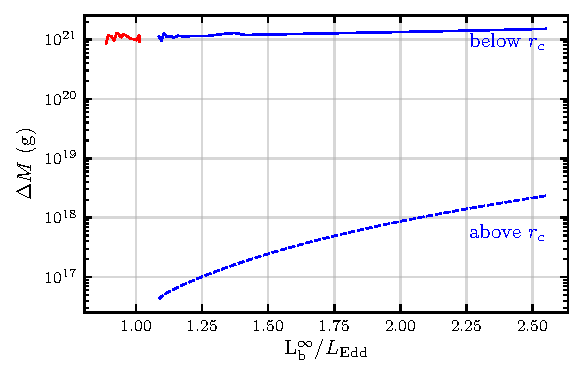
\includegraphics{figures/mass_contained.pdf}
    \caption[Mass stored in envelopes and winds]{Amount of mass stored in the envelopes (red) and the winds (blue), as a function of the base luminosity. For winds, we show the mass below (solid) and above (dashed) the critical point separately. The wiggle of the curves can be attributed to numerical interpolation \& integration errors.}
    \label{fig:mass_contained}
\end{figure}

\section{On the definition of the photosphere}\label{sec:compare_photosphere_def}
A limitation of our work is the pure optically thick approximation. While this approach, which consists of transporting heat under a diffusion equation (Eq.~\ref{eq:photondiffusion}), is completely valid in the inner layers of the extended structures, it becomes less so as we approach regions of low densities and temperatures, where the photons are no longer scattering purely isotropically but are instead, on average, increasingly beamed outwards. This is why we do not integrate our models past the photosphere, where the gas is becoming optically thin. In a pure optically thick treatment of radiation, this photosphere is hard to define. For expanded envelopes, hydrostatic equilibrium allows us to define a precise photosphere with a commonly used optical depth $\tau=2/3$. However in the outflowing wind case, we must resort to using a proxy for the true optical depth.  

In this work, we followed \citet{Paczynski1986b} by using the optical depth parameter value $\tau^*=\kappa\rho r=3$ to define the wind photosphere. Since we are making direct comparisons of the photospheric radii for the two regimes in Fig.~\ref{fig:triple}, we must ask whether or not these different definitions of photospheres are similar to each other. We cannot compute the location of $\tau=2/3$ in the wind models, but we can calculate $\tau^*$ in the envelopes, which we show in Fig.~\ref{fig:env_taustar}. The first thing we notice is the important difference between the most compact envelopes and the most extended ones. The compact envelopes have $\tau^*$ values larger than 3 at the photosphere. The extended ones have very small values of $\tau
^*$, even before the photosphere, which calls into question the validity of the optically thick approximation for these models. In any case, we already determined that these models were unlikely to be stable and exist in bursts, with their sound crossing times being so long.  

For the compact envelope models that are likely to exist at some point before or after the PRE phase, Fig.~\ref{fig:env_taustar} suggests that their photosphere, should the wind definition be taken instead of $\tau=2/3$, would be slightly larger than indicated in Fig.~\ref{fig:triple}. However, this would not change the fact that the transition between the two regimes is not smooth at the photosphere, and our conclusion that the transition is time-dependent remains valid. 

With Fig.~\ref{fig:env_taustar} showing that there is a considerable difference between $\tau$ and $\tau^*$ at the photosphere, there is a concern that the photospheres for some (or all) wind models is incorrectly defined. The only way to verify and fix this would be to add a transition to optically thin in our model and calculate new winds.  

\begin{figure}[htb!]
    \centering
    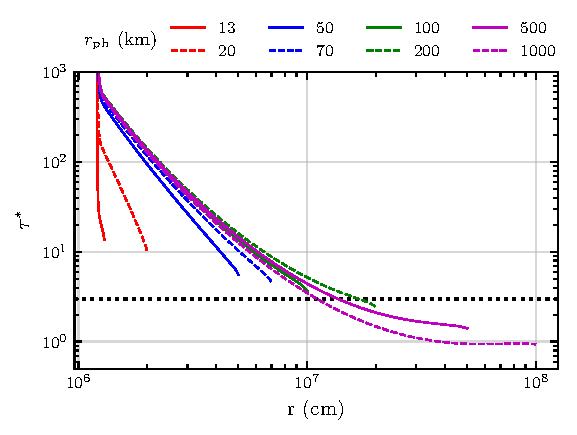
\includegraphics{figures/env_taustar.pdf}
    \caption[Optical depth parameter in the envelope models]{The optical depth parameter as a function of radius in the envelope models. The dotted black line marks the $\tau^*=3$ value used to define the wind photospheres.}
    \label{fig:env_taustar}
\end{figure}

\biblio
\end{document}
